
\newpage

\section{Light management}

One white global light illuminates the scene by default. This can be changed
through a light manager object and a certain number of lights (limited by
OpenGL).

The first step is to add the object called ``LightManager'', preferably at the
top of the scene file.
\begin{code_xml}
	<Object type=``LightManager'' />
\end{code_xml}

After that, we can add 3 different kinds of lights :
\begin{itemize}
  \item a positional light (parameters : color, position) ;
	\begin{figure}[!h]
	\centering
	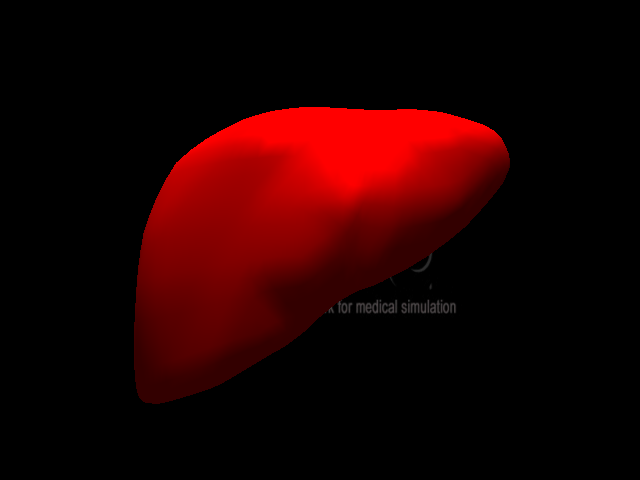
\includegraphics[width=0.33\linewidth]{rendering/images/light_pos.png}
	\caption{Positional Light}
	\end{figure}

	\begin{code_xml}
		<Object type="PositionalLight" position="0 -5 10" />
	\end{code_xml}
%\newpage
  \item a directional light (parameters : color, direction) ; 
	\begin{figure}[!h]
	\centering
	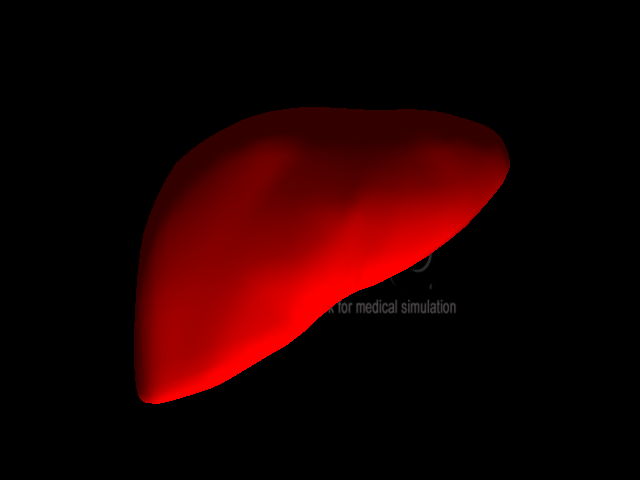
\includegraphics[width=0.33\linewidth]{rendering/images/light_dir.png}
	\caption{Directional Light}
	\end{figure}

	\begin{code_xml}
		<Object type="DirectionalLight" direction="0 5 0" />
	\end{code_xml}
\newpage

  \item and a spotlight (parameters : color, position, direction, cut off,
  exponent, attenuation)

	\begin{figure}[!h]
	\centering
	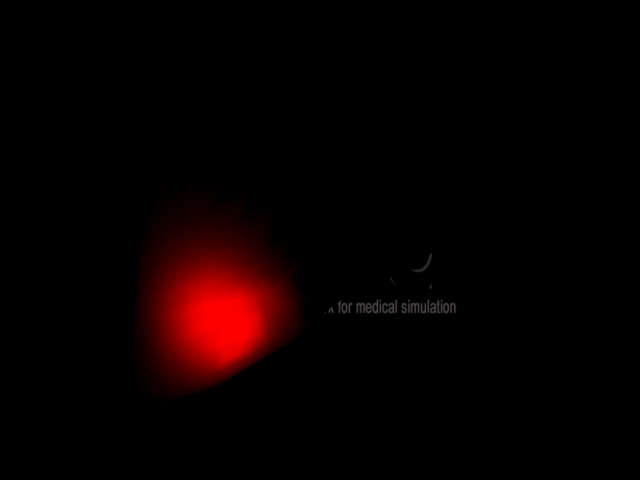
\includegraphics[width=0.33\linewidth]{rendering/images/light_spot.png}
	\caption{Spot Light}
	\end{figure}

	\begin{code_xml}
		<Object type="SpotLight" position="-3 2 5" direction="0 0 -1" />
	\end{code_xml}
\end{itemize}

\section{Shader management}
A complete set of tools about using shaders is implemented into SOFA. The three kinds of shaders (vertex and fragments (mandatory), geometry (optionally)) are available.
Shader is used only for Visual Model as OglModel.
\newline
The effects of the shader is spread to the associated subtree.
Finally, there is only one shader activated for each visual model : if two shaders are present in the same node, only the second will be effective.

	\begin{figure}[!h]
	\centering
	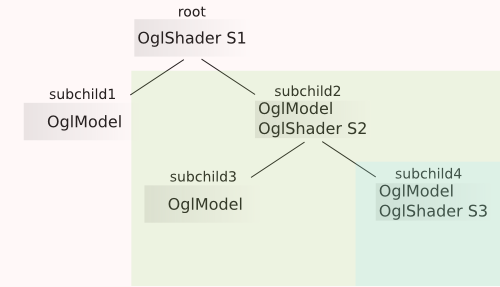
\includegraphics[width=0.8\linewidth]{rendering/images/shader_tree.png}
	\caption{Example of shaders' area of effect}
	\end{figure}

To simply include a shader, add this into your node :
	\begin{code_xml}
		<Object type="OglShader" vertFilename=``test.vert'' fragFilename=``test.frag'' />
	\end{code_xml}

\textit{vertFilename} and \textit{fragFilename} are the only mandatory parameters. Other optional parameters are about geometry shader : \textit{geoFilename}, \textit{geometryInputType}, \textit{geometryOutputType} and \textit{geometryVerticesOut}. A last parameter, \textit{turnOn}, is for debugging purpose, when you want to disable shader without restarting the scene.

If you want to send values to uniform variables defined into the shader, a certain number of objects is available : 
\begin{itemize}
 \item OglIntVariable,OglInt{2,3,4}Variable : for int and ivec{2,3,4}
 \item OglFloatVariable,OglFloat{2,3,4}Variable : for float and vec{2,3,4}
 \item OglIntVectorVariable, OglIntVector{2,3,4}Variable : for arrays of int and ivec{2,3,4}
 \item OglFloatVectorVariable, OglFloatVector{2,3,4}Variable : for arrays of float and vec{2,3,4}
\end{itemize}

Their parameters are \textit{id} for their name into the shader and \textit{value} (single type) or \textit{values} (array type).
Example : 
	\begin{code_xml}
		<Object type="OglFloat3Variable" id="fragmentColor" value="1.0 0.0 0.0" />
		<Object type="OglFloatVariable" id="fragmentOpacity" value="2.0"/>
		<Object type="OglFloatVector4Variable" id="MappingTable" values="1.0 0.0 0.0 0.0 0.0 0.0 0.0 1.0" />
	\end{code_xml}

2D texture can be added with OglTexture2D object.Its parameters are \textit{id}, \textit{texture2DFilename} and \textit {textureUnit}.

	\begin{code_xml} 
		<Object type="OglTexture2D" texture2DFilename="textures/lights4-small-noise.bmp" textureUnit="1" id="planeTexture" />
	\end{code_xml}

The last object about shaders is a partial support of macro processing in GLSL. It's possible to define macro variable if a part of code is enabled or not. For example, this can be very useful if there is a common code for two 3D objects, one with a texture, and the other with simple colors. You define the macro :

	\begin{code_cpp} 
		#define HAS_TEXTURE
			...;
			//code about textured 3D object
		#else
			...;
			//code about colored 3D object
		#endif
	\end{code_cpp}

and put the following object into the scene file, at the same node as the OglShader used by the textured 3D object:

	\begin{code_xml} 
		<Object type="OglShaderDefineMacro" id="HAS_TEXTURE" />
	\end{code_xml}


